\subsection{Finger grasping model}
At last, we have also to model the finger grasping the device, we can derive the model from the one used in \cite{Finger_grasping_model} for the human finger.

\begin{figure}
    \centering
    \resizebox{.9\linewidth}{!}{
        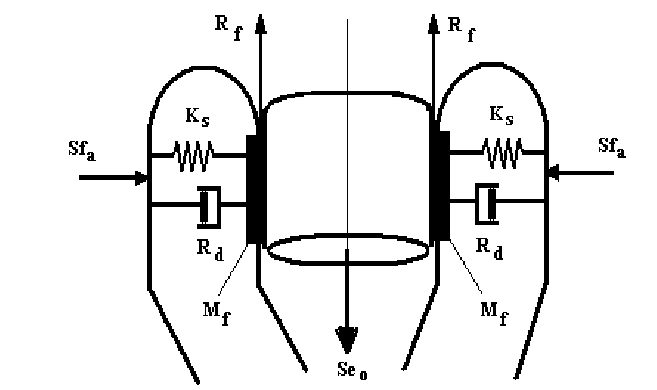
\includegraphics{Chapters/Chapter2/Modelling_of_Entire_System/Figures/Model-of-two-soft-fingers-grasping-the-object.png}
    }
    \caption{Model of two soft fingers grasping the object.}
    \label{fig: Finger grasping model}
\end{figure}

This model describes two fingers grasping an object, for our case, we can simplify it to a single finger grasping the device.
Also, we can neglect the friction between the finger and the device as the device will be tested positioned on a flat surface with only the finger touching it from above.
\begin{figure}
    \centering
    \resizebox{.9\linewidth}{!}{
        \begin{tikzpicture}
    \begin{scope}[every node/.style={bgelement}]
        \node (start) at (0,0) {};
        \node[right=1 of start] (w1) {1};
        \node[above=1 of w1] (Mf) {I: M\textsubscript{f}};
        \node[right=1 of w1] (v) {0};
        \node[above=1 of v] (w2) {1};
        \node[above=1 of w2] (Rdf) {R: Rd\textsubscript{f}};
        \node[right=1 of w2] (Cf) {C: $\frac{1}{Ks_{f}}$};
        \node[right=1 of v] (Sfa) {Sf\textsubscript{a}};
    \end{scope}
    \draw[bonds]
    (start) edge [e_out, flow={v}, effort={F}] (w1)
    (w1) edge [e_out] (Mf)
    (w1) edge [e_in] (v)
    (v) edge [e_in] (w2)
    (w2) edge [e_in] (Rdf)
    (w2) edge [e_in] (Cf)
    (Sfa) edge [e_out] (v);
\end{tikzpicture}
    }
    \caption{Bond graph of the finger grasping model.}
    \label{fig: Finger grasping bond graph}
\end{figure}
